\documentclass[11pt,a4paper]{article}


\usepackage[T1]{fontenc}
\usepackage[utf8]{inputenc}
\usepackage[margin=25mm]{geometry}
\usepackage{amsmath}
\usepackage{booktabs}
\usepackage{siunitx}
\usepackage{listings}
\usepackage{xcolor}
\usepackage{tikz}
\usepackage{caption}
\usepackage[expansion=false]{microtype}
\usepackage[hidelinks]{hyperref}

\usetikzlibrary{arrows.meta,positioning,calc}

\sisetup{per-mode=symbol, detect-weight=true}

\definecolor{codebg}{gray}{0.96}
\definecolor{codecom}{rgb}{0.20,0.45,0.20}
\definecolor{codekw}{rgb}{0.10,0.25,0.65}

\lstdefinelanguage{Simscape}{
  morekeywords={component,nodes,inputs,outputs,parameters,variables,branches,
    equations,events,when,elsewhen,else,end,if,assert,edge,der,abs,Event,true},
  sensitive=true,
  morecomment=[l]{\%},
  morestring=[b]',
}

\lstset{
  language=Simscape,
  basicstyle=\ttfamily\footnotesize,
  keywordstyle=\color{codekw}\bfseries,
  commentstyle=\color{codecom}\itshape,
  stringstyle=\color{black},
  backgroundcolor=\color{codebg},
  frame=single,
  rulecolor=\color{gray},
  breaklines=true,
  columns=fullflexible,
  showstringspaces=false,
  numbers=left,
  numberstyle=\tiny\color{gray},
  xleftmargin=6mm,
}

\newcommand{\code}[1]{\texttt{\small #1}}

\title{A Simplified Simscape IGBT Model with Single-Point Switching
Energies and Thermal Ports}
\author{Model documentation --- \code{igbt\_simple.ssc},
\code{igbt\_simple\_2th.ssc}}
\date{}

\begin{document}
\maketitle

\begin{abstract}
\noindent
This note documents a minimal Simscape language component that represents an
IGBT with its antiparallel free-wheeling diode (FWD) for loss and thermal
studies. Conduction is described by fixed voltage drops. Switching losses are
described by three single-point energies, $E_\mathrm{on}$, $E_\mathrm{off}$ and
$E_\mathrm{rr}$, given at one reference operating point and scaled linearly with
the commutated current and the blocking voltage. The total dissipated power is
delivered to one or two thermal conserving ports: a single-port version lumps
the two chips, a two-port version separates the transistor and the diode so
that the two junction temperatures can be evaluated independently. The document states the equations, the
sampling scheme used to recover the commutated current and voltage, the
energy-to-power conversion, the parameter extraction from the device datasheet,
and the validity limits of the model. Section~\ref{sec:2th} documents the two-port version, including the
local detection of the diode recovery event. Default parameters correspond to
the Mitsubishi Electric CM1200DW-34T (\SI{1700}{\volt}, \SI{1200}{\ampere}
half-bridge module).
\end{abstract}

\section{Scope and modelling assumptions}

The component is intended for system-level simulation of converters where the
quantities of interest are the average losses and the junction temperature, not
the shape of the switching transient. The following assumptions apply.

\begin{enumerate}
  \item The switching transient is not resolved in time. Each commutation is
        treated as an instantaneous event that injects a finite amount of energy
        into the thermal path. No $\mathrm{d}i/\mathrm{d}t$, no tail current and
        no reverse recovery current are visible on the electrical terminals.
  \item Conduction is represented by a fixed voltage drop. The output
        characteristic is therefore a vertical line in the $I$--$V$ plane, not
        the datasheet curve.
  \item All parameters are constant. In particular they do not depend on the
        junction temperature computed by the thermal network. The user is
        expected to enter the values corresponding to the expected operating
        temperature, typically \SI{125}{\degreeCelsius}.
  \item In the single-port version the IGBT and the FWD share one thermal
        port, so the model returns the total loss of one switch position and
        cannot separate the two junctions. The two-port version of
        Section~\ref{sec:2th} removes this restriction.
\end{enumerate}

Assumption~3 removes the electro-thermal feedback loop. This is a deliberate
simplification: it makes the model non-iterative and numerically robust, at the
cost of a loss estimate that is correct only near the chosen temperature. If the
simulated junction temperature departs significantly from the assumed one, the
parameters must be re-entered and the simulation repeated.

\section{Component interface}

\begin{table}[h]
\centering
\caption{Ports.}
\begin{tabular}{llll}
\toprule
Name & Type & Domain & Meaning \\
\midrule
\code{p} & conserving & electrical & collector \\
\code{n} & conserving & electrical & emitter \\
\code{H} & conserving & thermal & case/junction heat flow \\
\code{g} & input & physical signal & gate--emitter voltage, \si{\volt} \\
\code{P} & output & physical signal & total instantaneous loss, \si{\watt} \\
\bottomrule
\end{tabular}
\end{table}

\noindent
The port side declared in the trailing comment of a node declaration accepts
\code{left} and \code{right}; \code{top} and \code{bottom} are not accepted for
this component and cause a compilation error.

\begin{table}[h]
\centering
\caption{Parameters and default values (CM1200DW-34T).}
\begin{tabular}{llll}
\toprule
Symbol & Name & Default & Source \\
\midrule
$V_\mathrm{ce,sat}$ & \code{Vce\_sat} & \SI{2.40}{\volt} &
  typ.\ at \SI{1200}{\ampere}, \SI{125}{\degreeCelsius}, terminal \\
$V_\mathrm{f}$ & \code{Vf} & \SI{2.80}{\volt} &
  $V_\mathrm{EC}$ typ.\ at \SI{1200}{\ampere}, \SI{125}{\degreeCelsius} \\
$V_\mathrm{th}$ & \code{Vth} & \SI{6}{\volt} & $V_\mathrm{GE(th)}$ typ. \\
$V_\mathrm{hyst}$ & \code{Vhyst} & \SI{0.85}{\volt} & user choice \\
$E_\mathrm{on,ref}$ & \code{Eon\_ref} & \SI{138}{\milli\joule} &
  table value, see Sec.~\ref{sec:param} \\
$E_\mathrm{off,ref}$ & \code{Eoff\_ref} & \SI{309}{\milli\joule} &
  table value, see Sec.~\ref{sec:param} \\
$E_\mathrm{rr,ref}$ & \code{Err\_ref} & \SI{220}{\milli\joule} &
  table value, see Sec.~\ref{sec:param} \\
$I_\mathrm{c,ref}$ & \code{Ic\_ref} & \SI{1200}{\ampere} & test condition \\
$V_\mathrm{dc,ref}$ & \code{Vdc\_ref} & \SI{1000}{\volt} & test condition \\
$R_\mathrm{on}$ & \code{Ron} & \SI{0.05}{\milli\ohm} & numerical \\
$R_\mathrm{d}$ & \code{Rd} & \SI{0.05}{\milli\ohm} & numerical \\
$G_\mathrm{off}$ & \code{Goff} & \SI{1}{\micro\siemens} & numerical \\
$\tau_\mathrm{s}$ & \code{tau\_s} & \SI{1}{\micro\second} & numerical \\
$\tau_\mathrm{p}$ & \code{tau\_p} & \SI{200}{\micro\second} & numerical \\
\bottomrule
\end{tabular}
\end{table}

\section{Conduction}

Let $v = v_\mathrm{p} - v_\mathrm{n}$ be the terminal voltage and $i$ the
terminal current flowing from \code{p} to \code{n}. The terminal current is
split into a transistor current $i_\mathrm{t}$ and a diode current
$i_\mathrm{d}$,
\begin{equation}
  i = i_\mathrm{t} + i_\mathrm{d},
\end{equation}
each governed by a piecewise linear characteristic:
\begin{align}
  i_\mathrm{t} &=
  \begin{cases}
    \dfrac{v - V_\mathrm{ce,sat}}{R_\mathrm{on}}, &
      g > V_\mathrm{th} \ \wedge\ v > V_\mathrm{ce,sat},\\[2mm]
    G_\mathrm{off}\, v, & \text{otherwise},
  \end{cases}
  \label{eq:it}\\[2mm]
  i_\mathrm{d} &=
  \begin{cases}
    \dfrac{v + V_\mathrm{f}}{R_\mathrm{d}}, & v < -V_\mathrm{f},\\[2mm]
    G_\mathrm{off}\, v, & \text{otherwise}.
  \end{cases}
  \label{eq:id}
\end{align}

The two series resistances are not intended as a physical model of the output
characteristic. They exist to make each conduction mode an explicit, invertible
relation between $v$ and $i$: a strictly fixed voltage drop would impose
$v = V_\mathrm{ce,sat}$ as an algebraic constraint independent of current, and
the mode selection at current reversal would become implicit, which is a common
source of chattering. With $R_\mathrm{on} = \SI{0.05}{\milli\ohm}$ the extra
drop at \SI{1200}{\ampere} is \SI{60}{\milli\volt}, i.e.\ \SI{2.5}{\percent} of
$V_\mathrm{ce,sat}$.

If a more faithful conduction model is wanted, $R_\mathrm{on}$ and $R_\mathrm{d}$
can be set to the slope of the datasheet output characteristic and
$V_\mathrm{ce,sat}$, $V_\mathrm{f}$ to the corresponding zero-current
intercepts. This turns \eqref{eq:it}--\eqref{eq:id} into the usual
$v = V_0 + R\,i$ representation at no extra cost.

The off-state conductance $G_\mathrm{off}$ closes the mesh when the device is
blocking. Both branches contribute, so the leakage current at
\SI{1200}{\volt} is \SI{2.4}{\milli\ampere} and the associated blocking loss is
\SI{2.9}{\watt}. This is of the same order as the datasheet $I_\mathrm{CES}$
limit and is negligible with respect to the other loss terms; $G_\mathrm{off}$
may be reduced if a smaller residual is preferred, at the price of a larger
resistance ratio and a stiffer network.

The gate input is compared with the threshold $V_\mathrm{th}$. The model
therefore accepts a gate signal expressed in volts, and a driver output swinging
between $-V_\mathrm{GE}$ and $+V_\mathrm{GE}$ can be fed directly.

\section{Switching losses}

\subsection{Scaling law}

The three energies are given at a single reference point
$(I_\mathrm{c,ref}, V_\mathrm{dc,ref})$ and scaled bilinearly:
\begin{equation}
  E_x(I,V) = E_{x,\mathrm{ref}}\,
             \frac{|I|}{I_\mathrm{c,ref}}\,
             \frac{|V|}{V_\mathrm{dc,ref}},
  \qquad x \in \{\mathrm{on},\mathrm{off},\mathrm{rr}\}.
  \label{eq:scaling}
\end{equation}
The dependence on the blocking voltage is close to linear for a hard-switched
IGBT, so the second factor is a good approximation over the usual DC-link range.
The dependence on current is not exactly linear: the datasheet curves of
$E_\mathrm{on}$ and $E_\mathrm{off}$ versus $I_\mathrm{C}$ are slightly convex,
and $E_\mathrm{rr}$ saturates at high current. Equation~\eqref{eq:scaling}
therefore over-estimates the energy at low current and under-estimates it near
the rated current if the reference point is taken at rated current. Choosing the
reference point near the expected average commutated current, rather than at the
datasheet rated point, reduces this error.

\subsection{Recovering the commutated current and voltage}

The quantities to be inserted in \eqref{eq:scaling} are the current that the
device commutates and the voltage it blocks. Neither is available at the
switching instant itself:

\begin{itemize}
  \item at turn-on the pre-event voltage is the blocking voltage, but the
        pre-event current is zero;
  \item at turn-off the pre-event current is the conducted current, but the
        pre-event voltage is $V_\mathrm{ce,sat}$.
\end{itemize}

Moreover, the value that the solver associates with a continuous variable inside
an event equation is not guaranteed to be the pre-transition one, so sampling
$v$ and $i$ directly in the \code{when} clause is unreliable.

The model avoids the problem by never sampling at the event. Two continuous
first-order states track the required quantities during the intervals in which
they are meaningful, and hold them otherwise:
\begin{align}
  \dot{i}_\mathrm{h} &=
  \begin{cases}
    \dfrac{i_\mathrm{t} - i_\mathrm{h}}{\tau_\mathrm{s}}, & g > V_\mathrm{th},\\[2mm]
    0, & \text{otherwise},
  \end{cases}
  \label{eq:ih}\\[2mm]
  \dot{v}_\mathrm{h} &=
  \begin{cases}
    \dfrac{v - v_\mathrm{h}}{\tau_\mathrm{s}}, & g < V_\mathrm{th} \ \wedge\ v > 0,\\[2mm]
    0, & \text{otherwise}.
  \end{cases}
  \label{eq:vh}
\end{align}

Because $i_\mathrm{h}$ and $v_\mathrm{h}$ are continuous states, they cannot jump
at an event; whatever the solver does with $v$ and $i$ at the transition, the
held values are the pre-transition ones. With
$\tau_\mathrm{s} \ll t_\mathrm{on,min}$ the tracking error is negligible.

The scheme has a useful side effect. At turn-on, $i_\mathrm{h}$ contains the
transistor current measured just before the \emph{previous} turn-off. For
$f_\mathrm{sw} \gg f_\mathrm{out}$ this is the load current to be commutated,
which is exactly what \eqref{eq:scaling} requires. If instead the diode was
conducting during the previous on-state, then $i_\mathrm{t} \approx 0$ was
tracked and $i_\mathrm{h} \approx 0$, so the model assigns
$E_\mathrm{on} \approx 0$. This is the correct behaviour: an IGBT turning on
while its own antiparallel diode carries the load current does not commutate
current and dissipates almost nothing.

\begin{figure}[h]
\centering
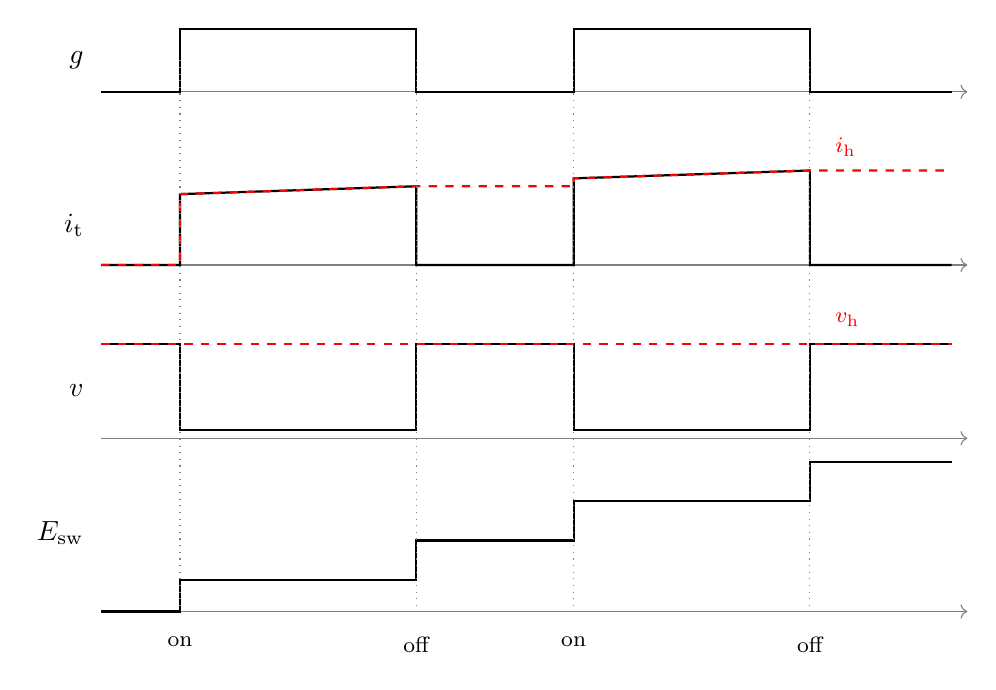
\begin{tikzpicture}[x=1mm,y=1mm]
  \def\rowsep{22}
  % --- gate ---
  \draw[->,gray] (0,0) -- (110,0);
  \draw[thick] (0,0) -- (10,0) -- (10,8) -- (40,8) -- (40,0) -- (60,0)
               -- (60,8) -- (90,8) -- (90,0) -- (108,0);
  \node[anchor=east] at (-1,4) {$g$};
  % --- transistor current ---
  \begin{scope}[yshift=-\rowsep mm]
  \draw[->,gray] (0,0) -- (110,0);
  \draw[thick] (0,0) -- (10,0) -- (10,9) -- (40,10) -- (40,0) -- (60,0)
               -- (60,11) -- (90,12) -- (90,0) -- (108,0);
  \draw[thick,dashed,red] (0,0) -- (10,0) -- (10,9) -- (40,10) -- (60,10)
                          -- (60,11) -- (90,12) -- (108,12);
  \node[anchor=east] at (-1,5) {$i_\mathrm{t}$};
  \node[red,anchor=west,font=\footnotesize] at (92,15) {$i_\mathrm{h}$};
  \end{scope}
  % --- terminal voltage ---
  \begin{scope}[yshift=-2*\rowsep mm]
  \draw[->,gray] (0,0) -- (110,0);
  \draw[thick] (0,12) -- (10,12) -- (10,1) -- (40,1) -- (40,12) -- (60,12)
               -- (60,1) -- (90,1) -- (90,12) -- (108,12);
  \draw[thick,dashed,red] (0,12) -- (108,12);
  \node[anchor=east] at (-1,6) {$v$};
  \node[red,anchor=west,font=\footnotesize] at (92,15) {$v_\mathrm{h}$};
  \end{scope}
  % --- energy staircase and filtered power ---
  \begin{scope}[yshift=-3*\rowsep mm]
  \draw[->,gray] (0,0) -- (110,0);
  \draw[thick] (0,0) -- (10,0) -- (10,4) -- (40,4) -- (40,9) -- (60,9)
               -- (60,14) -- (90,14) -- (90,19) -- (108,19);
  \node[anchor=east] at (-1,10) {$E_\mathrm{sw}$};
  \end{scope}
  % markers
  \foreach \x in {10,40,60,90} {
    \draw[gray,dotted] (\x,4) -- (\x,-3*\rowsep);
  }
  \node[font=\footnotesize,anchor=north] at (10,-3*\rowsep-2) {on};
  \node[font=\footnotesize,anchor=north] at (40,-3*\rowsep-2) {off};
  \node[font=\footnotesize,anchor=north] at (60,-3*\rowsep-2) {on};
  \node[font=\footnotesize,anchor=north] at (90,-3*\rowsep-2) {off};
\end{tikzpicture}
\caption{Sampling scheme. The held current $i_\mathrm{h}$ freezes at turn-off
and is reused at the following turn-on; the held voltage $v_\mathrm{h}$ freezes
at turn-on and is reused at the following turn-off. Each event adds a step to
the cumulative energy $E_\mathrm{sw}$.}
\end{figure}

\subsection{Event equations}

The two commutations are written as a single \code{when}/\code{elsewhen} chain
acting on one event variable $E_\mathrm{sw}$:
\begin{align}
  E_\mathrm{sw} &\leftarrow E_\mathrm{sw}
    + \bigl(E_\mathrm{on,ref} + E_\mathrm{rr,ref}\bigr)
      \frac{|i_\mathrm{h}|}{I_\mathrm{c,ref}}
      \frac{|v_\mathrm{h}|}{V_\mathrm{dc,ref}}
    && \text{on } g \uparrow (V_\mathrm{th} + V_\mathrm{hyst}),\\
  E_\mathrm{sw} &\leftarrow E_\mathrm{sw}
    + E_\mathrm{off,ref}
      \frac{|i_\mathrm{h}|}{I_\mathrm{c,ref}}
      \frac{|v_\mathrm{h}|}{V_\mathrm{dc,ref}}
    && \text{on } g \downarrow (V_\mathrm{th} - V_\mathrm{hyst}).
\end{align}

Two separate \code{when} clauses updating the same event variable are rejected
by the compiler, because it cannot prove that the two predicates are mutually
exclusive. The \code{elsewhen} form makes exclusivity structural. The hysteresis
band $V_\mathrm{hyst}$ around $V_\mathrm{th}$ prevents multiple events on a noisy
or slow gate edge; the gate waveform must cross both thresholds, otherwise
events are missed and the switching loss is under-estimated.

\subsection{Attribution of the recovery energy}

The reverse recovery energy of a diode is dissipated when the diode is
commutated off by the turn-on of the \emph{complementary} switch of the same
leg. That instant is not observable from the terminals of a single
switch-position model. The model therefore charges $E_\mathrm{rr}$ to the
turn-on event of its own transistor, together with $E_\mathrm{on}$.

In a two-device leg made of identical instances this preserves the total leg
loss exactly and misplaces only its distribution: the pair
$E_\mathrm{on} + E_\mathrm{rr}$ appears at the switch that turns on, instead of
$E_\mathrm{on}$ at that switch and $E_\mathrm{rr}$ at the diode of the opposite
one. Since the present model already lumps the IGBT and its FWD onto one thermal
port, the additional error concerns only the split between the upper and lower
positions of a leg, which is symmetric over a fundamental period. If the diode
is modelled as a separate component with its own recovery energy,
$E_\mathrm{rr,ref}$ must be set to zero here to avoid double counting.

This approximation is acceptable only as long as the two chips share one
thermal port. As soon as the junction temperatures are computed separately it
becomes a real error, because the recovery energy would be assigned to the
diode during the half period in which that diode does not conduct, flattening
exactly the peak that the calculation is meant to find. The two-port version
therefore detects the recovery event locally; see Section~\ref{sec:2th}.

\section{From energy steps to dissipated power}

$E_\mathrm{sw}$ is a staircase. Its derivative is a train of Dirac impulses,
which cannot be injected into a thermal network. The model converts the
staircase into power with a first-order lag. Let
\begin{equation}
  \dot{E}_\mathrm{lp} = \frac{E_\mathrm{sw} - E_\mathrm{lp}}{\tau_\mathrm{p}},
  \qquad
  P_\mathrm{sw} = \frac{E_\mathrm{sw} - E_\mathrm{lp}}{\tau_\mathrm{p}}
                = \dot{E}_\mathrm{lp}.
  \label{eq:lag}
\end{equation}
A step of height $\Delta E$ occurring at $t_k$ produces
\begin{equation}
  P_\mathrm{sw}(t) = \frac{\Delta E}{\tau_\mathrm{p}}\,
                     e^{-(t-t_k)/\tau_\mathrm{p}},
  \qquad
  \int_{t_k}^{\infty} P_\mathrm{sw}\,\mathrm{d}t = \Delta E .
\end{equation}
The energy is therefore conserved exactly; only its distribution in time is
smoothed. Over an interval containing $N$ events,
\begin{equation}
  \int_{0}^{T} P_\mathrm{sw}\,\mathrm{d}t
  = E_\mathrm{lp}(T) - E_\mathrm{lp}(0)
  = \sum_{k=1}^{N}\Delta E_k
    - \bigl[E_\mathrm{sw}(T) - E_\mathrm{lp}(T)\bigr],
\end{equation}
and the residual term is bounded by $\tau_\mathrm{p}P_\mathrm{sw}(T)$, i.e.\ by
the energy of roughly one time constant of switching loss. In steady state the
mean of $P_\mathrm{sw}$ equals $f_\mathrm{sw}\bigl(E_\mathrm{on} +
E_\mathrm{off} + E_\mathrm{rr}\bigr)$, as it should.

The total instantaneous loss delivered to the thermal port is
\begin{equation}
  P = \underbrace{v\,i}_{\text{conduction}} + P_\mathrm{sw}.
\end{equation}

\subsection{Choice of $\tau_\mathrm{p}$}

$\tau_\mathrm{p}$ must satisfy two conflicting requirements. It should span
several switching periods, so that the power seen by the thermal network is a
smooth average rather than a sequence of spikes, and it should stay below the
smallest thermal time constant that is to be resolved. For the reference module
the fastest Foster stage has $\tau_1 = \SI{19.6}{\micro\second}$, which is
shorter than a switching period at any realistic $f_\mathrm{sw}$ for a
\SI{1200}{\ampere} device: the junction temperature ripple inside a switching
period is not resolvable with averaged losses in any case, and
$\tau_\mathrm{p}$ of a few switching periods is the appropriate choice. The
default \SI{200}{\micro\second} corresponds to a few periods at
$f_\mathrm{sw} = \SIrange{2}{5}{\kilo\hertz}$. Junction temperature swings at
the output fundamental frequency, which are usually the quantity of interest,
are unaffected as long as $\tau_\mathrm{p} \ll 1/f_\mathrm{out}$.

\section{Thermal port}

The thermal port is declared as a conserving node and its heat flow is bound in
the \code{branches} section:
\begin{lstlisting}
branches
    i : p.i -> n.i;
    Q : H.Q -> *;
end
\end{lstlisting}
The balancing variable \code{H.Q} may only be referenced in \code{branches};
using it directly in \code{equations} is a compilation error. With the
declaration above, $Q$ is positive when heat flows \emph{into} the component,
so the dissipation is imposed as
\begin{equation}
  Q = -P .
\end{equation}
The equivalent form \code{Q : * -> H.Q} together with $Q = +P$ is also valid.

The component contains no thermal capacitance and no thermal resistance: it is a
pure heat source. The junction-to-case impedance must be attached externally.
For the reference module the datasheet gives a four-stage Foster network in
normalised form, which becomes, for the IGBT
($R_\mathrm{th(j-c)Q} = \SI{28}{\kelvin\per\kilo\watt}$):

\begin{table}[h]
\centering
\caption{Foster network derived from the normalised transient thermal impedance
data, IGBT chip.}
\begin{tabular}{cS[table-format=1.3]S[table-format=2.3]S[table-format=1.3]S[table-format=1.3]}
\toprule
$k$ & {$r_k$ (--)} & {$R_k$ (\si{\milli\kelvin\per\watt})} &
{$\tau_k$ (\si{\second})} & {$C_k$ (\si{\joule\per\kelvin})} \\
\midrule
1 & 0.0124 & 0.347  & 0.0000196 & 0.056 \\
2 & 0.0739 & 2.069  & 0.00140   & 0.677 \\
3 & 0.3510 & 9.828  & 0.0179    & 1.821 \\
4 & 0.5630 & 15.764 & 0.0944    & 5.988 \\
\bottomrule
\end{tabular}
\end{table}

\noindent
with $R_k = r_k R_\mathrm{th(j-c)Q}$ and $C_k = \tau_k/R_k$. The same
normalised coefficients apply to the FWD with
$R_\mathrm{th(j-c)D} = \SI{43}{\kelvin\per\kilo\watt}$. Because the single-port
model has one thermal port, one network must be chosen for the pair; using the
IGBT network is the usual choice when the IGBT carries the larger share of the
loss. The two-port version uses both networks, one per port.

\section{Parameter extraction from the datasheet}
\label{sec:param}

Two points deserve attention when the parameters are taken from a datasheet.

\paragraph{Temperature.} The tabulated switching energies of the reference
module are specified at $T_\mathrm{vj} = \SI{150}{\degreeCelsius}$, whereas the
conduction voltages are tabulated at \SI{25}{\degreeCelsius},
\SI{125}{\degreeCelsius} and \SI{150}{\degreeCelsius}. A parameter set that is
consistent at \SI{125}{\degreeCelsius} therefore requires reading the energies
from the dashed curves rather than from the table. For the reference module the
resulting values at \SI{1200}{\ampere} are approximately
\SI{130}{\milli\joule}, \SI{285}{\milli\joule} and \SI{205}{\milli\joule} for
$E_\mathrm{on}$, $E_\mathrm{off}$ and $E_\mathrm{rr}$, i.e.\ some
\SIrange{5}{10}{\percent} below the tabulated \SI{150}{\degreeCelsius} figures.
These are graphical readings and should be treated as such.

\paragraph{Gate resistance.} The tabulated energies are measured at
$R_\mathrm{G} = \SI{0}{\ohm}$, which is not an operating condition. The
datasheet curves of switching energy versus external gate resistance show a
strong dependence: at the maximum recommended turn-on resistance of
\SI{6.8}{\ohm} the turn-on energy is roughly an order of magnitude larger than
at $R_\mathrm{G} = \SI{0}{\ohm}$, while the recovery energy decreases and the
turn-off energy roughly doubles at the maximum recommended turn-off resistance
of \SI{15}{\ohm}. Entering the tabulated values without correcting for the
actual gate resistance leads to a gross under-estimate of the turn-on loss. The
energies must be read at the gate resistance of the actual driver.

\section{Variant with separate thermal ports}
\label{sec:2th}

The component \code{igbt\_simple\_2th} keeps the equations of
Sections~3--5 unchanged and splits the loss into two independent paths, one per
chip. It adds two thermal ports, \code{Ht} for the transistor and \code{Hd} for
the diode, two power outputs \code{Pt} and \code{Pd}, and one parameter,
$V_\mathrm{rr,th}$ (default \SI{50}{\volt}), used to detect the recovery event.

\subsection{Loss split}

Conduction separates naturally, since the two branch currents are already
distinct state variables of the model. The switching energies are accumulated in
two event variables, $E_\mathrm{t}$ for the transistor and $E_\mathrm{d}$ for
the diode, each with its own first-order lag:
\begin{align}
  P_\mathrm{t} &= v\,i_\mathrm{t}
    + \frac{E_\mathrm{t} - E_\mathrm{lp,t}}{\tau_\mathrm{p}},
  & E_\mathrm{t} &\ \text{fed by } E_\mathrm{on},\ E_\mathrm{off},\\
  P_\mathrm{d} &= v\,i_\mathrm{d}
    + \frac{E_\mathrm{d} - E_\mathrm{lp,d}}{\tau_\mathrm{p}},
  & E_\mathrm{d} &\ \text{fed by } E_\mathrm{rr}.
\end{align}
The two heat flows are bound to the two ports as
$Q_\mathrm{t} = -P_\mathrm{t}$ and $Q_\mathrm{d} = -P_\mathrm{d}$ with the sign
convention of Section~6.

\subsection{Local detection of the recovery event}

The instant at which the diode is commutated off is imposed by the
complementary switch of the leg and is not directly observable from the
terminals of a single switch position. It is, however, observable indirectly:
it is the only instant at which the terminal voltage rises from the diode
conduction level to the blocking level while the transistor is not the cause of
the transition. The model therefore triggers on
\begin{equation}
  v \uparrow V_\mathrm{rr,th},
  \qquad V_\mathrm{f} < V_\mathrm{rr,th} \ll V_\mathrm{dc},
\end{equation}
and scales $E_\mathrm{rr}$ with a held diode current $i_\mathrm{dh}$ governed by
a three-branch law:
\begin{equation}
  \dot{i}_\mathrm{dh} =
  \begin{cases}
    \dfrac{|i_\mathrm{d}| - i_\mathrm{dh}}{\tau_\mathrm{s}},
      & v < -V_\mathrm{f} \quad\text{(diode conducting: track)},\\[3mm]
    -\dfrac{i_\mathrm{dh}}{\tau_\mathrm{s}},
      & g > V_\mathrm{th} \quad\text{(transistor gated on: flush)},\\[3mm]
    0, & \text{otherwise \quad(dead time: hold)}.
  \end{cases}
  \label{eq:idh}
\end{equation}

The flush branch is what makes the detection self-selecting. The voltage rise
above $V_\mathrm{rr,th}$ occurs once per switching period in both half periods
of the output fundamental, but only in one of them does it correspond to a
recovery, and \eqref{eq:idh} guarantees that $i_\mathrm{dh}$ is non-zero only in
that one. Table~\ref{tab:halfperiods} follows the two cases.

\begin{table}[h]
\centering
\caption{Behaviour of the recovery detection over the two half periods of the
output current, for one switch position.}
\label{tab:halfperiods}
\begin{tabular}{lll}
\toprule
 & Diode half period & Transistor half period \\
\midrule
Chip carrying the load current & FWD & IGBT \\
Branch of \eqref{eq:idh} in the on-state & track & flush \\
$i_\mathrm{dh}$ during the dead time & held & $\approx 0$ \\
Cause of the voltage rise & complementary turn-on & own turn-off \\
Energy added at the event & $E_\mathrm{rr}(i_\mathrm{dh})$ & $\approx 0$ \\
\bottomrule
\end{tabular}
\end{table}

The hold branch covers the dead time: the gate is already low while the diode is
still conducting, and the current must not be lost before the commutation
actually happens. The order of the branches matters, because during the
freewheeling interval the gate of the switch position is typically high while
the current flows in the diode; testing the diode conduction first ensures that
this interval is tracked and not flushed.

\subsection{Event chain}

The three events are written as a single \code{when}/\code{elsewhen} chain:
\begin{lstlisting}
events
    when edge(g > (Vth + Vhyst))
        E_t = E_t + Eon_ref *(abs(i_h) /Ic_ref)*(abs(v_h)/Vdc_ref);
    elsewhen edge(g < (Vth - Vhyst))
        E_t = E_t + Eoff_ref*(abs(i_h) /Ic_ref)*(abs(v_h)/Vdc_ref);
    elsewhen edge(v > V_rr_th)
        E_d = E_d + Err_ref *(abs(i_dh)/Ic_ref)*(abs(v_h)/Vdc_ref);
    end
end
\end{lstlisting}
The chain form is required for the same reason as in the single-port version:
separate \code{when} clauses acting on the same event variable are rejected
because their predicates cannot be proved mutually exclusive. In the transistor
half period the turn-off predicate and the voltage-rise predicate become true
almost simultaneously; whether the solver resolves them in one or in two event
iterations is immaterial, since the recovery term is zero there.

\subsection{Thermal connection}

Each port takes its own junction-to-case network, built from the normalised
Foster coefficients of Section~6 scaled with
$R_\mathrm{th(j-c)Q} = \SI{28}{\kelvin\per\kilo\watt}$ for \code{Ht} and
$R_\mathrm{th(j-c)D} = \SI{43}{\kelvin\per\kilo\watt}$ for \code{Hd}. Both
networks are connected to a common case node, followed by
$R_\mathrm{th(c-s)} = \SI{10}{\kelvin\per\kilo\watt}$ per module and by the
heatsink model. The internal nodes of a Foster network have no physical
meaning, but its terminal behaviour reproduces the datasheet $Z_\mathrm{th}$,
and connecting both chips to a shared case node is the usual practice.

\subsection{Use in a dimensioning calculation}

With the two ports available, the peak junction temperature of each chip
becomes a direct simulation output. Two points are worth checking explicitly.

First, the peak depends on the output frequency. At low fundamental frequency
the thermal ripple over a half period becomes dominant and is not captured by
the average loss: the transient at the lowest fundamental frequency of the duty
profile, not the mean value, is the sizing case.

Second, the diode is not necessarily the less critical chip. It carries the full
load current during a half period, its junction-to-case resistance is
significantly higher than that of the transistor, and its recovery loss is
concentrated in the same half period in which it conducts. A FWD with a lower
average loss than the IGBT can therefore reach a higher peak junction
temperature, which is precisely the effect that the single-port version, and the
approximate attribution of $E_\mathrm{rr}$, would hide.

\section{Validity limits}

The model does not represent:
\begin{itemize}
  \item the switching transient, hence no $\mathrm{d}v/\mathrm{d}t$ or
        $\mathrm{d}i/\mathrm{d}t$ stress, no overshoot due to stray inductance,
        no tail current and no recovery current on the electrical terminals;
  \item the temperature dependence of the conduction drops and of the switching
        energies;
  \item the dependence of the switching energies on the gate resistance, the
        stray inductance and the DC-link decoupling;
  \item the difference between IGBT and FWD junction temperatures, in the
        single-port version only;
  \item any short-circuit, desaturation or avalanche behaviour;
  \item the non-linearity of the output characteristic, unless $R_\mathrm{on}$
        and $R_\mathrm{d}$ are set to the datasheet slopes.
\end{itemize}

Within these limits the model reproduces the loss balance of a hard-switched
converter with the accuracy of the datasheet data themselves, at a computational
cost close to that of an ideal switch. Validation against a vendor loss
calculator, at fixed junction temperature and identical gate resistance, is the
recommended acceptance test.

\appendix
\section{Source listings}

\subsection{Single thermal port}
\lstinputlisting{igbt_simple.ssc}

\subsection{Separate thermal ports}
\lstinputlisting{igbt_simple_2th.ssc}

\end{document}
